\documentclass[a4paper]{article}
\usepackage[14pt]{extsizes} % для того чтобы задать нестандартный 14-ый размер шрифта
\usepackage[margin=0.7in]{geometry}
\usepackage{multirow}
\usepackage {graphicx}
\usepackage[utf8x]{inputenc} % указать кодировку русского текста
\usepackage[russian]{babel} % указать, что язык текста - русский
\usepackage{fancyhdr}
\pagestyle{fancy}
\usepackage{graphicx}
\graphicspath{{pictures/}}
\DeclareGraphicsExtensions{.pdf,.png,.jpg, .jpeg}
\usepackage{tocloft}
\usepackage{wrapfig}
\usepackage{tikz}
\renewcommand{\cftsecleader}{\cftdotfill{\cftdotsep}}
\begin{document} 
 \begin{titlepage}
\begin{center}
\hfill \break
Министерство науки и высшего образования Российской Федерации\\
ФЕДЕРАЛЬНОЕ ГОСУДАРСТВЕННОЕ АВТОНОМНОЕ ОБРАЗОВАТЕЛЬНОЕ\\ 
УЧРЕЖДЕНИЕ ВЫСШЕГО ОБРАЗОВАНИЯ\\ 
«МОСКОВСКИЙ ФИЗИКО-ТЕХНИЧЕСКИЙ ИНСТИТУТ\\ 
(НАЦИОНАЛЬНЫЙ ИССЛЕДОВАТЕЛЬСКИЙ УНИВЕРСИТЕТ)»\\
(МФТИ)\\
\hfill \break
\hfill \break
\hfill \break
\hfill \break
\hfill \break
\hfill \break
\hfill \break
\hfill \break
\hfill \break
\hfill \break
\hfill \break
ЛАБОРАТОРНАЯ РАБОТА 4.3.1\\
\hfill \break
ИЗУЧЕНИЕ ДИФРАКЦИИ СВЕТА\\
\end{center}
\hfill \break
\hfill \break
\hfill \break
\hfill \break
\hfill \break
\hfill \break
\hfill \break
\hfill \break
\hfill \break
\hfill \break
\begin{tabular}{ccc}
Работу выполнила студентка группы Б01-009 & & М.В.Шлапак \\\\
\end{tabular}
\hfill \break
\hfill \break
\hfill \break
\hfill \break
\hfill \break
\hfill \break
\hfill \break
\hfill \break
\begin{center} Долгопрудный 2022 \end{center}
\end{titlepage}
\small
\fancyhead[L] {Изучение дифракции света}
\tableofcontents    
\newpage
\section{Аннотация к работе}

В работе предстоит исследовать явления дифракции Френеля и Фраунгофера на одной щели, дифракции Фраунгофера на двух щелях, изучить влияние дифракции на разрешающую способность оптических приборов.

\section{Теоретические сведения}
\subsection{Дифракция Френеля}
\begin{figure}[h]
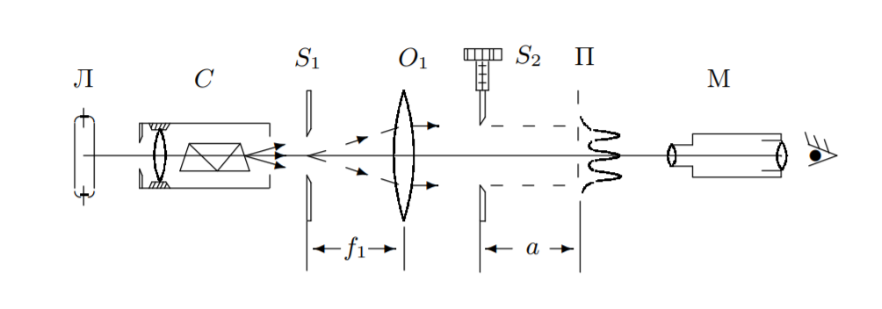
\includegraphics[width=0.7\textwidth]{1.png}
\centering
\caption{Схема установки.}
\end{figure}
Распределение интенсивности света в плоскости П рассчитаем с помощью зон Френеля. При освещении $S_2$ параллельным пучком лучей (плоская зона) зоны Френеля представляют собой плоскости, параллельные краям щели. Результирующая амплитуда в точке наблюдения определеяется суперпозицией колебаний от тех зон Френеля, которые не перекрыты створками щели. Графическое определение результирующей амплитуды производится с помощью векторной диаграммы -- спирали Корню. Суммарная ширина $m$ зон Френеля $z_m$ определяется соотношение
\begin{equation}
z_m = \sqrt{am\lambda},
\end{equation}
где $a$ -- расстояние от щели до плоскости П. Вид наблюдаемой картины определяется \textit{числом Френеля} $\Phi$:
$$
\Phi^2 = \frac{D}{\sqrt{a\lambda}}
$$
-- число зон Френеля, которые укладываются в ширине щели $D$. $p = \frac{1}{\Phi^2}$ называется \textit{волновым параметром}. 
\subsection{Дифракция Фраунгофера на одной щели}

\begin{wrapfigure}{r}{0.5\textwidth}
  \begin{center}
    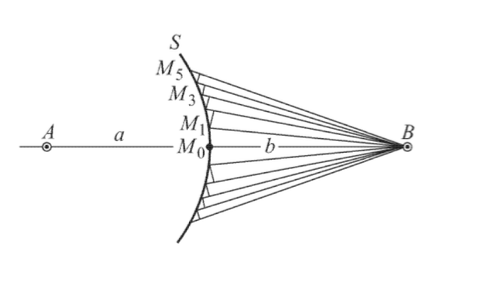
\includegraphics[width = 0.4\textwidth]{2.png}
  \end{center}
  \caption{Построение зон Френеля}
\end{wrapfigure}
Для выкладок ниже нам потребуется знать \textit{принцип Гюйгенса-Френеля}. Он формулируется следующим образом 

\textit{Каждый элемент волнового фронта можно рассматривать как центр  вторичного возмущения, порождающего вторичные сферические волны, а результирующее световое поле  в каждой точке пространства будет определяться интерференцией этих волн.}

Теперь рассмотрим первое применение этого принципа, получившее название \textit{метод зон Френеля}

Для этого рассмотрим действие световой волны действующей из точки $A$ в какой-то точке $B$.

В этом случае можно, взяв точку $M_0$ в качестве центра (см. рис. 1), построить ряд концентрических сфер, радиусы которых начинаются с $b$ и увеличиваются каждый раз на половину длины волны $\lambda/2$. При пересечении с плоским фронтом волны $F$ эти сферы дадут концентрические окружности. Таким образом, на фронте волны появятся кольцевые зоны (зоны Френеля) с радиусами $r_1, r_2$ и т. д.

Из геометрических соображений посчитав, можно получить, что 
\begin{equation}
r_i = i \sqrt{a \lambda}
\end{equation}	
Введем так же обозначение: \textit{число Френеля}
\begin{equation}
\Phi^2 = \frac{D}{\sqrt{a\lambda}}
\end{equation}
\begin{wrapfigure}{r}{0.5\textwidth}
  \begin{center}
    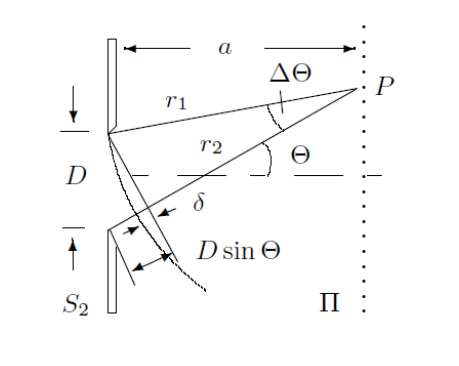
\includegraphics[width = 0.3\textwidth]{3.png}
  \end{center}
  \caption{К фазовым соотношениям при дифракции Фраунгофера}
\end{wrapfigure}
В этом пункте рассмотрим дифракцию, когда ширина щели становится значительно меньше ширины первой зоны Френеля, т.е. если 
\begin{equation}
D \ll\sqrt{a \lambda} 
\end{equation}	
Это условие всегда выполняется при достаточно большом $a$. В этом случае говорят, что \textit{дифракция Фраунгофера}. При выполнении пункта $(2)$ у нас заметно упрощаются фазовые соотношения, что поясняет рис. 3, в итоге с хорошим приближением можно считать, что разность хода между соседними лучами равна 
\begin{equation}
\Delta = r_2 - r_1 \approx D \sin \theta \approx D \cdot \theta
\end{equation}
Здесь предполагается, что $\theta$ достаточно мал.
\subsection*{Схема установки}
Дифракцию Фраунгофера можно наблюдать на подобной установке 

\begin{figure}[h]
\begin{center}
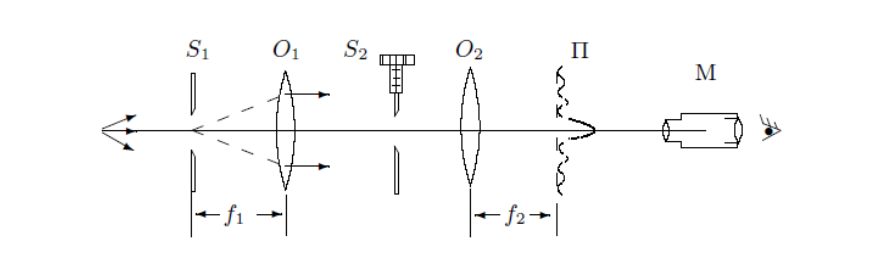
\includegraphics[width = 0.7\textwidth]{4.png}
\caption{Схема установки для пункта 2}
\end{center}
\end{figure}

Объектив здесь нужен для удобства, так как неудобно работать с очень узкими щелями. Дифракционная картина здесь наблюдается в фокальной плоскости объектива $O_2$. 

Посчитав легко определить угловую координату любой темной полосы:
\begin{equation}
\theta_m = \frac{m \lambda}{b}
\end{equation}
И расстояние от центра соответственно 
\begin{equation}
X_m = f_2m\frac{\lambda}{b}
\end{equation}

\subsection{Дифракция Фраунгофера на двух щелях}

Заменим $S_2$ на две щели 

\begin{figure}[h]
\begin{center}
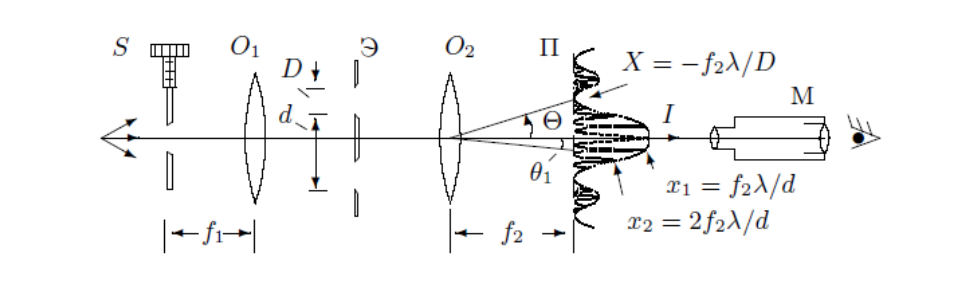
\includegraphics[width = 0.8\textwidth]{5.png}
\caption{Установка для третьего пункта}
\end{center}
\end{figure}

В этом случае легко видеть, что угловая координата максимума будет: 
\begin{equation}
\theta_m = \frac{m \lambda}{d}
\end{equation}
И между соседними полосами:
\begin{equation}
\delta x = f_2 \frac{\lambda}{d}
\end{equation}
Также нетрудно оценить число интерференционных полос укладывающихся в области центрального максимума: 
\begin{equation}
n = \frac{2d}{b}
\end{equation}
\subsection{Влияние дифракции на разрешающую способность оптического инструмента}

\begin{figure}[h]
\begin{center}
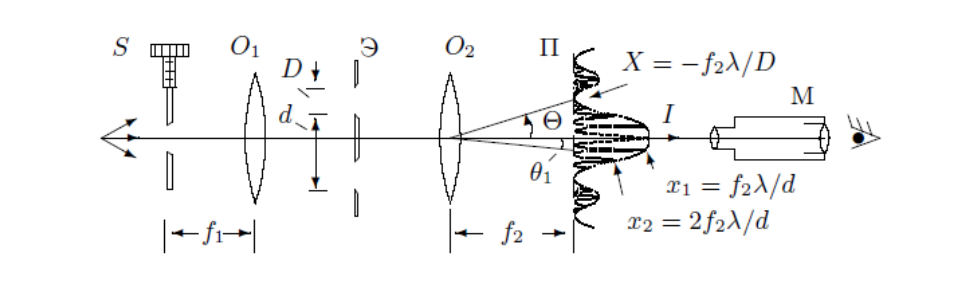
\includegraphics[width = 0.8\textwidth]{5.png}
\caption{Схема установки для пункта 4.}
\end{center}
\end{figure}

Если перед $O_2$ расположить $S_2$, то изображение объекта будет искажено из-за дифракции. Качественной характеристикой этого искажения может служить $\varphi_{min}$ --- минимальное угловое между объектами (источниками). 

\begin{equation}
\varphi = \frac{d}{f_1}
\end{equation}
Из геометрии $l$ между объектами равно 
\begin{equation}
l = \phi \cdot d_2
\end{equation}
\begin{equation}
\frac{\lambda}{D_0} = \frac{l}{f_2} = \frac{d}{f_1}
\end{equation}

\newpage
\section{Результаты измерений и обработка данных}
\subsection{А. Дифракция Френеля на щели}
\subsection*{Настройка установки}
Соберём схему, согласно описанию в лабораторной работе. Убеждаемся, что луч идёт вдоль оптической скамьи. Далее настроим пучок света на параллельность. Для этого установим линзу O1 на расстоянии от щели S1, близком к фокусному расстоянию $F_1 = 16$ см. Более точную настройку получим при помощи зрительной трубы, настроенной на бесконечность: слегка перемещая линзу O1 вдоль оптической скмьи, добьемся чёткого изображения входной щели S1 в зрительной трубе.\\
Далее определим нуль микрометрического винта щели S2, чтобы в дальнейшем учитывать его при измерении размера щели S2 с помощью микрометра. \\
\em Нуль микрометрического винта: $+30$ делений (цена деления - $0,001$ мм)\em \\
Далее фокусируем микроскоп на поставленную за линзой О1 щель S2. Перемещая микроскоп вдоль оптической скамьи, добьемся чёткого изображения щели S2, причём при небольшом удалении от этого положения в окуляре появляются узкие чёрные полосы, количество которых уменьшается по мере удаления микроскопа. Таким образом, получаем дифракцию в ближней волновой зоне (дифракция Френеля).
\subsection*{Измерения}
Добившись наибольшей чёткости дифракционной картины, снова найдем резкое изображение щели (чёткие края без дифракционных полос). Запишем начальное положение микроскопа - координату по шкале продольной линейки, расположенной на оптической скамье. \\
\em Начальное положение микроскопа: $x_0 = 45,8$ см\em \\
Постепенно отодвигая микроскоп от щели $S2$, снимем зависимость координаты микроскопа $z_n$ (смещение микроскопа от первоначального положения) от числа $n$ наблюдаемых тёмных полос:\\
\\
\begin{center}
\begin{tabular}{|l|l|l|}
\hline
n & $x_n$, см & $z_n$, см\\
\hline
1 & 43 & 2,8 \\
\hline
2 & 44 & 1,8\\
\hline
3 & 44,5 & 1,3\\
\hline
4 & 44,8 & 1\\
\hline
5 & 45 & 0,8\\
\hline
\end{tabular}
\end{center}
Измерим ширину $b$ щели S2 двумя способами: с помощью шкалы микроскопа и с помощью микрометра:\\
$$b_1 = 0,30 \pm 0,01 \; mm$$
$$b_2 = 0,330 \pm 0,001 \; mm$$
Видно, что расхождения получились не слишком большие: более точное измерение (с помощью микрометра) находится в полосе $3\sigma$ менее точного измерения.\\
\subsection*{Качественные наблюдения}
Получим \em дифракцию Френеля на препятствии \em : для этого поставим вместо щели S2 рамку с тонкой вертикальной нитью. Настроим микроскоп на резкое изображение нити и убедимся, что при удалении микроскопа от нити на её фоне всегда наблюдается чётное число тёмных дифракционных полос (центр светлый).\\
\\
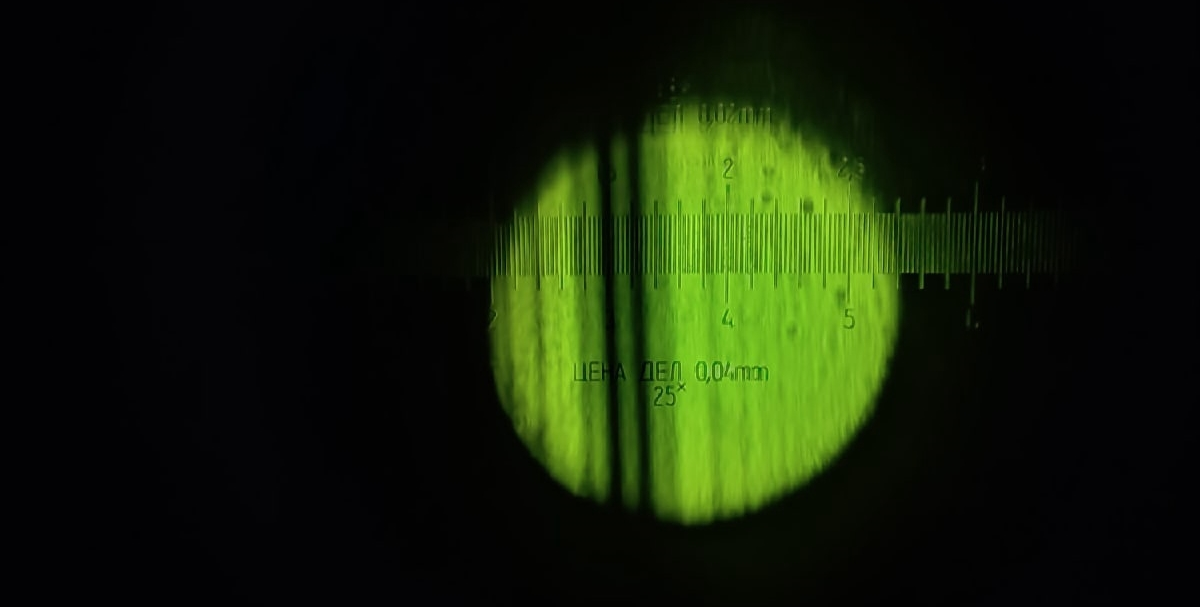
\includegraphics[width=18cm]{a1}\\
\subsection*{Обработка результатов}
Оценим по порядку волновой параметр $p = \frac{\sqrt{z \lambda}}{b}$, чтобы убедиться, что рассматриваемая нами дифракция действительно является дифракцией Френеля.\\
$$ p \propto \frac{\sqrt{10^{-2} \; m \cdot 500 \cdot 10^{-9}\; m}}{10^{-4} \; m} \approx  0,7$$
Сравним размер открытых зон Френеля с измеренной шириной $b$ щели S2. Для этого свяжем число тёмных полос $n$ в поле зрения с числом зон Френеля $m$ на полуширине щели, где суммарная ширина зон Френеля (Шустера) рассчитывается по формуле: \\
$$\xi_n = \sqrt{zn\lambda}$$
\begin{center}
\begin{tabular}{|l|l|l|l|l|l|}
\hline
n & $x_n$, см & $z_n$, см & $2\xi$, мкм & $\sigma_{\xi}$, мкм & $\sigma_{x}$, см\\
\hline
1 & 43 & 2,8 & 254 &2&0,05 \\
\hline
2 & 44 & 1,8 & 288 & 4&0,05 \\
\hline
3 & 44,5 & 1,3 & 300 & 6&0,05 \\
\hline
4 & 44,8 & 1 & 304 & 8& 0,05\\
\hline
5 & 45 & 0,8 & 305 & 10& 0,05\\
\hline
\end{tabular}
\end{center}
Погрешности в таблице выше получаются для $x$ из половины цены деления поперечных салазок микроскопа (было описано в пункте 3), а для $z_m$ из почленного дифференцирования формулы $(1)$, а именно погрешность для $z_m$ равна 
$$ \sigma_{2\xi} = \sqrt{(\frac{\delta (2\sqrt{zn\lambda})}{\delta z})^2}\sigma_z$$


Усреднив $2\xi_n$ мы получим ширину щели $b$, погрешность для нее считается по формуле :
$$ \sigma_b = \frac{1}{\sqrt{n(n-1)}} \cdot \sqrt{\sum\limits_{i=1}^n (b_i - b)^2}$$
Таким образом, значения для ширины щели:
$$ b_{theor} = 0,29 \pm 0,09 \; mm$$ 
$$ b_{prac} = 0,30 \pm 0,01 \; mm$$
Построим график $2\xi_n = f(n)$, отложим на нём величину $b$. За $\lambda$ в нашем эксперименте принимается длина волны жёлтой линии ртути: $\lambda = 578$ нм.\\
\\
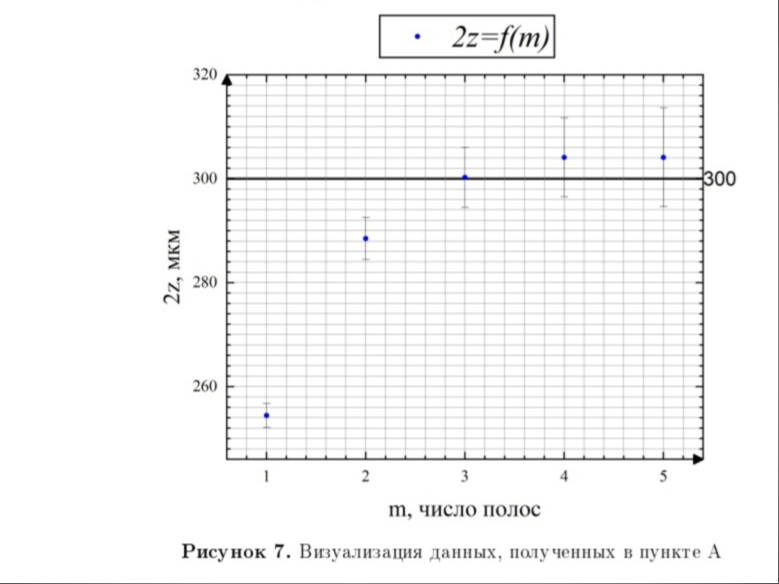
\includegraphics[width=18cm]{a2}
\section{Б. Дифракция Фраунгофера на щели}
\subsection*{Настройка установки}
Для перехода из ближней волновой зоны (дифракция Френеля) в дальнюю (дифракция Фраунгофера) к установке, собранной в пункте А, достаточно добавить линзу О2 (рис.4)\\
Аналогично пункту А настраиваем параллельность пучка за линзой О1. Настроив микроскоп на фокальную плоскость линзы, уменьшением ширины щели S1 проверяем, что микроскоп настроен на края щели. Ширину щели S2 при этом подбираем такой, чтобы в поле зрения микроскопа появилась дифракционная картина. В отличие от френелевой дифракционной картины фраунгоферова занимает всё поле зрение микроскопа.\\
\subsection*{Измерения}
Измерим с помощью окулярной шкалы микроскопа координаты $x_m$ нескольких дифракционных минимумов ( от -m до +m):\\
\begin{center}
\begin{tabular}{|l|l|l|l|}
\hline
m & $x_{min}$, мм & $x_{max}$, мм & $x_m$, мм\\
\hline
-2 &1,54 & 1,62 & 1,58\\
\hline
-1 & 1,86 & 1,92 & 1,89\\
\hline
+1 & 2,44 & 2,50 & 2,47\\
\hline
+2 & 2,72 & 2,86 & 2,79\\
\hline
\end{tabular}
\end{center}
$\sigma_m = 0$, $\sigma_{x_{min}} = \sigma_{x_{max}} = 0,01$ мм, $\sigma_x = 0,014 \approx 0,01$ мм\\
\\
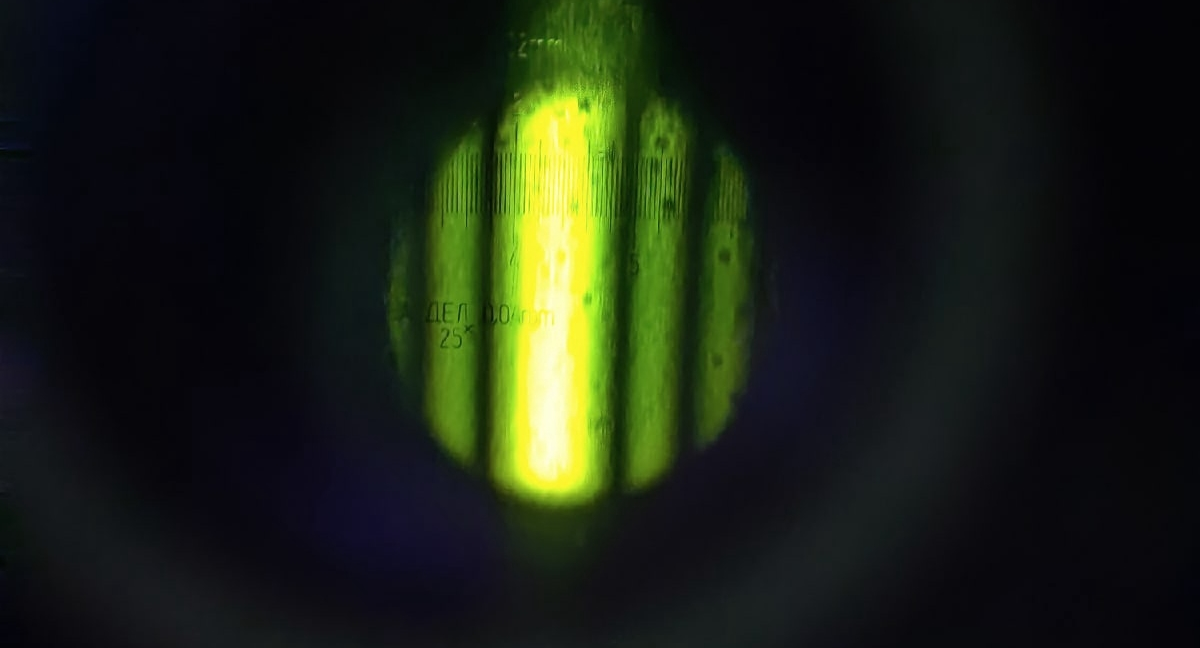
\includegraphics[width=18cm]{b1}\\
\subsection*{Качественные наблюдения}
Убедились на практике в том, что смещение щели S2 в боковом направлении не приводит к сдвигу дифракционной картины.\\
\subsection*{Обработка результатов}
Оценим по порядку волновой параметр $p = \frac{\sqrt{z \lambda}}{b}$, чтобы убедиться, что рассматриваемая нами дифракция действительно является дифракцией Фраунгофера.\\
$$ p \propto \frac{\sqrt{10^{-1} \; m \cdot 500 \cdot 10^{-9}\; m}}{10^{-4} \; m} \approx 2,23$$
Построим график, откладывая по горизонтали номер минимума $m$, а по вертикали - его координату $x_m$. По углу наклона прямой определим среднее расстояние между соседними минимумами ($\Delta x_m/2m = x_m/m$). Рассчитаем ширину щели $b$ по формуле ниже и сравним с измеренной:
$$x_m = m\frac{\lambda}{b}f_2$$
\begin{center}
\begin{tabular}{|l|l|l|l|l|l|}
\hline
m & $x_{min}$, мм & $x_{max}$, мм & $x_m$, мм & $b$, мм & $\sigma_b$, мм\\
\hline
-2 &1,54 & 1,62 & 1,58 & 0,94 & 0,19\\
\hline
-1 & 1,86 & 1,92 & 1,89 & 0,39 & 0,04\\
\hline
+1 & 2,44 & 2,50 & 2,47 & 0,30 &0,02 \\
\hline
+2 & 2,72 & 2,86 & 2,79 & 0,53 & 0,03\\
\hline
\end{tabular}
\end{center}
$\sigma_m = 0$, $\sigma_{x_{min}} = \sigma_{x_{max}} = 0,01$ мм, $\sigma_x = 0,014 \approx 0,01$ мм\\
Погрешность вычисления $b$, как и в пункте А, бралась как погрешность функции от нескольких переменных. \\
Усредним значения $b$ и получаем:
$$b_{theor} = 0,246 \pm 0,013 \; mm$$
$$b_{prac} = 0,282 \pm 0,001 \; mm$$
Достаточно большую погрешность ($50 \%$) можно объяснить малым количеством экспериментальных измерений (мы получили всего 4 минимума).\\
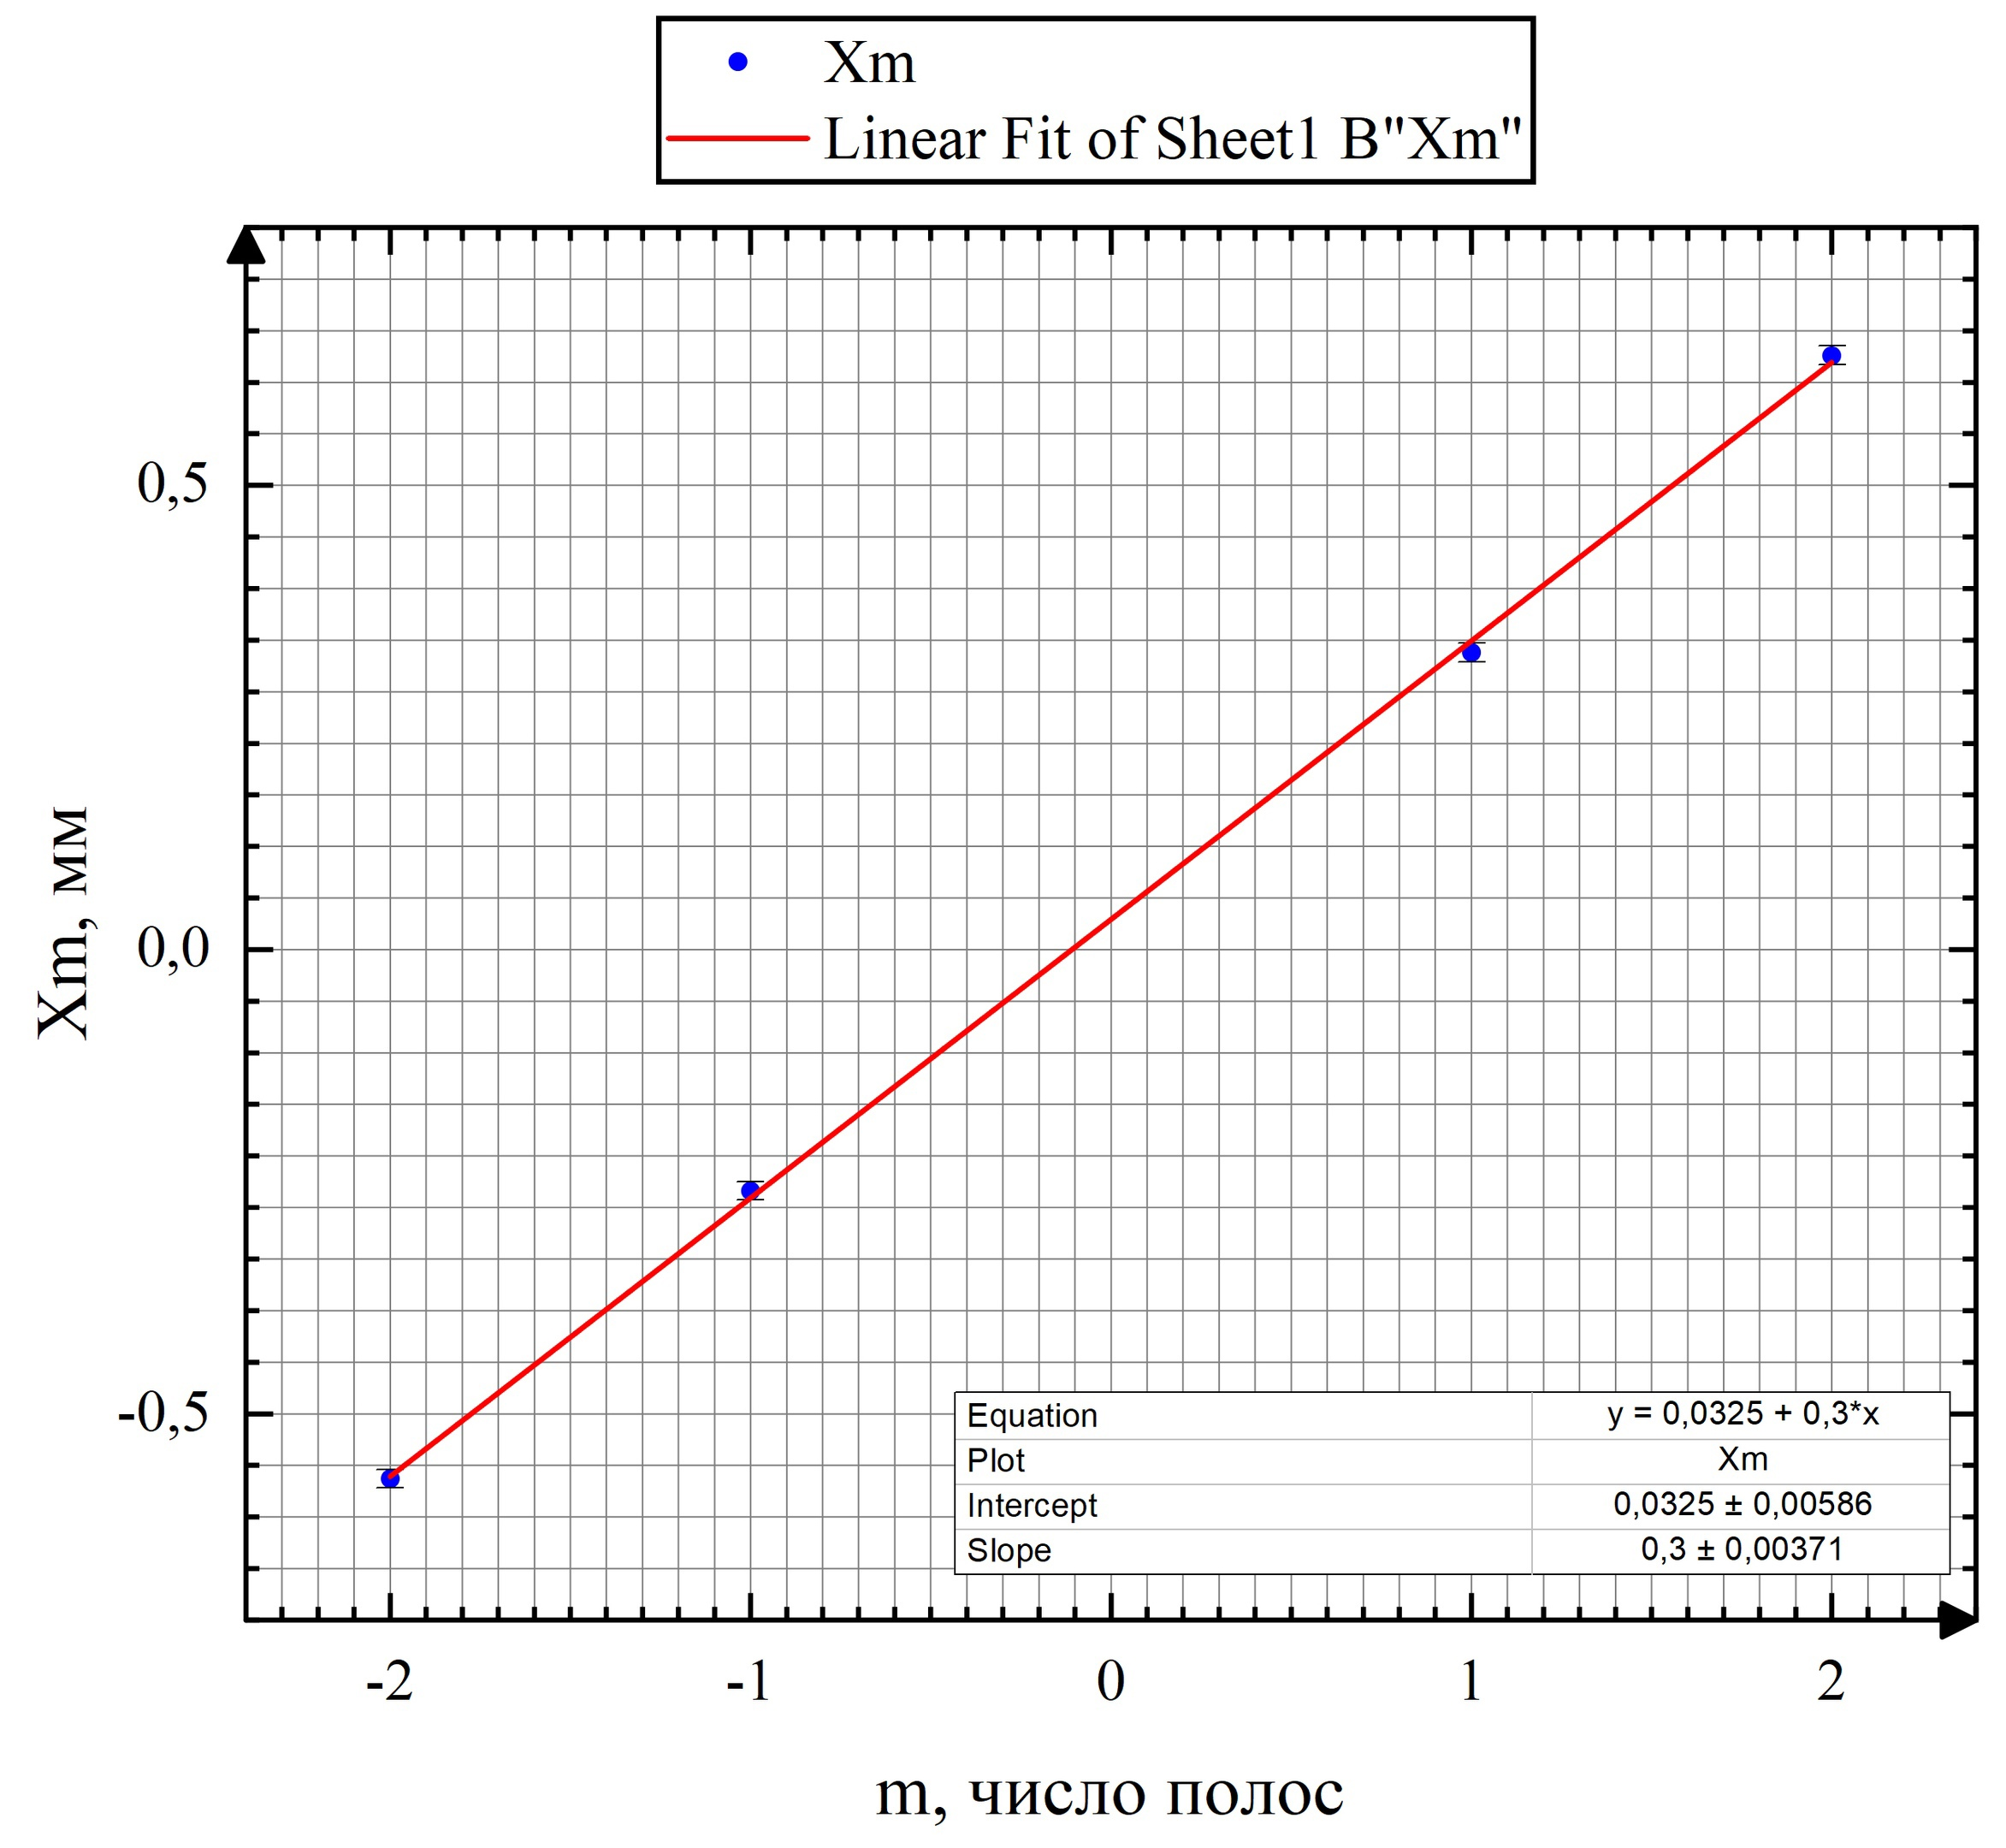
\includegraphics[width=18cm]{b2}\\
Так как наклон графика получился $k = 1,282 \pm 0,314$ мм, то $\Delta x \approx 0,3 \pm 0,004$ мм\\
\section{В. Дифракция Фраунгофера на двух щелях}
\subsection*{Настройка и измерения}
Заменив в установки из пункта Б входную щель S1 щелью с микрометрическим винтом и, слегка передвигая её вдоль скамьи, найдем в микроскопе резкое изображение новой входной щели. Ставим между линзами экран Э с двойной вертикальной щелью. В области главного дифракционного максимума должна появиться система равноотстоящих темных и светлых полос. Добьемся наибольшей чёткости получившейся дифракционной картины.\\
Определим с помощью окулярной шкалы координаты самых удаленных друг от друга темных полос внутри центрального максимума и просчитаем число светлых промежутков между ними. Измерим также ширину центрального максимума.
\begin{center}
Самая правая полоса: $1,58 \pm 0,01$ мм\\
Самая левая полоса: $1,14 \pm 0,01$ мм\\
Число светлых промежутков между полосами: $9$\\
Ширина центрального максимума: $0,44 \pm 0,01$ мм\\
\end{center}
Исследуем влияние пространственной когерентности на видность интерференционной картины. Для этого, расширяя входную щель S, подберем такую ширину щели $b_0$, при которой наступает первое исчезновение интерференционных полос:
$$b_0 \approx 0,074 \pm 0,01 \; mm$$
Запишем фокусные расстояния обеих линз:
\begin{center}
$F_1 = 16$ см\\
$F_2 = 12,5$ см\\
\end{center}
\subsection*{Обработка результатов}
Определим расстояние $\delta x$ между минимумами по результатам измерений, рассчитаем величину $d$ по формуле $\delta x = f_2 \frac{\lambda}{d}$ и сравним с измеренной экспериментально.\\
$$\delta x = \frac{x}{n} \approx 49 \pm 6 \; mkm$$
Здесь погрешность берется из формулы
	$$\sigma_d =  \sqrt{\left(\frac{\partial \left(f_2 \frac{\lambda}{\delta x}  \right)}{\partial \left(\delta x\right)}\right)^{2} \cdot \sigma_{\delta x}^2} = f_2\lambda \frac{1}{\delta x^2} \cdot \sigma_{\delta x}$$

	Измерив мы получили, что 
	$$d = 1,5 \pm 0,2 \; mm$$
	$$b = 0,33 \pm 0,01 \; mm$$
	Погрешность берем как половину цены деления.
	Отсюда мы получаем, что
	$$n_{theor} = 9 \pm 1$$
$n$ рассчитывалось по формуле:
$$ n = \frac{2d}{b}$$
	Погрешность для $n$ берем из формулы 
	$$\sigma_n =\sqrt{\left(\frac{\partial \frac{2d}{b}}{\partial d}\right)^{2} \cdot \sigma_{d}^2 + \left(\frac{\partial \frac{2d}{b}}{\partial b}\right)^{2} \cdot \sigma_{b}^2} = \sqrt{\frac{4\sigma_d^2}{b^2} + \frac{4d^2\sigma_{b}^2}{b^4}}$$
Исследуем влияние когерентности на видность картины. Для этого расширяя щель $S$ подберём $b_0$ такую, при которой первый раз исчезают интерференционные полосы. $b_{0} = (0,074 \pm 0,001)$ мм. Из формулы 
	$$\frac{b}{f_1} = \frac{\lambda}{d}$$
	мы получаем, что 
	$$b_{theor} = 0,063 \pm 0,001 \; mm$$
	Погрешность для этой формулы опять таки берется из
	$$\delta b = \left|\frac{\partial \frac{f_1 \lambda}{d}}{\partial d}\right| \sigma_d = \frac{b f_1 \lambda}{d^2} \cdot \sigma_d = \frac{b^2\sigma_d}{d}$$

\section{Г. Влияние дифракции на разрешающую способность оптического инструмента}
В этом пункте исследуем влияние размера диафрагмы, ограничивающей поперечный размер пучка света, на чёткость изображения объекта.\\
\subsection*{Настройка и измерения}
Поставим вместо щели S экран с двойной щелью и, перемещая его вдоль оптической оси, получим в поле зрения микроскопа чёткое, симметричное изображение двойного источника.\\
Поставим между линзами щель S2 и, уменьшая её ширину, наблюдаем ухудшение качества изображения. Подберём ширину щели S2 так, чтобы изображения обеих щелей почти сливались, но всё-таки еще воспринимались раздельно. Запишем показания микрометрического винта щели S2 $b_0$:\\
$$b_0 = 0,088 \pm 0,001 \; mm$$
Поставим двойную щель перед микроскопом и измерим с помощью окулярной шкалы расстояние $d$ между щелями и ширину каждой щели $b$:
$$d = 1,780\pm 0,001 \; mm$$
$$b = 0,260 \pm 0,001 \; mm$$
\subsection*{Обработка реузльтатов}
Проверим справедливость критерия Рэлея, для этого сравним измеренную ширину $b_0$ щели S2 с расчётом по формуле $b_0 = \frac{\lambda}{d}f_1$\\
$$b_{0theor} = 0,052 \pm 0,001 \; mm$$
Погрешность рассчитывалась по формуле из пункта В.
\section{Выводы:}
Приведем итоги наших вычислений в таблице:\\
	\begin{tabular}{|c|c|c|c|c|}
		\hline
		& \begin{tabular}[c]{@{}c@{}}Дифракция \\ Френеля\end{tabular} & \begin{tabular}[c]{@{}c@{}}Дифракция \\ Фраунгофера\\ на одной щели\end{tabular} &                 & \begin{tabular}[c]{@{}c@{}}Дифракция \\ Фраунгофера\\ на двух щелях\end{tabular} \\ \hline
		$b_{theor}$, мм & $0,29\pm 0,01$                                                          & $0,246 \pm 0,14$                                                                            & $b_{theor}$, мм & $0,063\pm0,001$                                                                             \\ \hline
		$b_{prac}$, мм  & $0,30\pm 0,01$                                                        & $0,28\pm 0,01$                                                                            & $b_{prac}$, мм  & $0,074\pm0,001$                                                                             \\ \hline
	\end{tabular}\\
	\\
Из нее мы видим, что все теоретические формулы, приведенные в данной работе хорошо сходятся с измерениями. \\
Так же в работе были проверены и подтверждены качественные рассуждения.
\end{document}